\documentclass[conference]{IEEEtran}
\IEEEoverridecommandlockouts
% The preceding line is only needed to identify funding in the first footnote. If that is unneeded, please comment it out.
%\usepackage{cite}
\usepackage[portuges,brazil,english]{babel}
\usepackage[utf8]{inputenc}
\usepackage{hyperref}
\usepackage{amsmath,amssymb,amsfonts}
\usepackage{amsmath}
\usepackage{algorithm}
\usepackage{algorithmic}
\usepackage{graphicx}
\usepackage{textcomp}
\DeclareUnicodeCharacter{00A0}{ }
\def\BibTeX{{\rm B\kern-.05em{\sc i\kern-.025em b}\kern-.08em
    T\kern-.1667em\lower.7ex\hbox{E}\kern-.125emX}}
\begin{document}

\title{Algoritmos genéticos aplicados ao Tetris}

\author{\IEEEauthorblockN{André Almeida}
\IEEEauthorblockA{
RA: 164047}
\and
\IEEEauthorblockN{Igor Torrente}
\IEEEauthorblockA{
RA: 169820}
\and
\IEEEauthorblockN{Lucas Cunha}
\IEEEauthorblockA{
RA: 172655}
\and
\IEEEauthorblockN{João Spuri}
\IEEEauthorblockA{
RA: 155943}}


\maketitle

\section{Resumo}
Nesse projeto, foram realizados estudos envolvendo técnicas de algoritmos genéticos em redes neurais artificiais para encontrar uma solução aproximada para um algoritmo que faça jogadas ideais no jogo \textit{Tetris}.

\section{Introdução}

\subsection{Tetris}
\subsubsection{O jogo}
Tetris é um jogo eletrônico criado em 1984 pelo matemático soviético Alexey Pazhitnov, tendo obtido grande popularidade principalmente nas plataformas \textit{Atari  ST} e no \textit{Nintendo Entertainment System} \cite{b1}. Até hoje, já foram vendidas mais de 50 milhões de cópias mundialmente. O jogo é do gênero \textit{puzzle}, onde o jogador precisa resolver algum tipo de quebra-cabeça. \\
No Tetris, o "tabuleiro" do jogo é formado por uma malha de 22\textit{x}10 quadrados (com as duas linhas do topo ocultas ao jogador), onde o jogador deve ir encaixando as peças (os "Tetraminós") que caem verticalmente no tabuleiro em uma sequência aleatória. Existem 7 tipos de Tetraminós, cada um formato distinto. O objetivo do jogador é manipular essas peças, movendo-as horizontalmente e girando-as de forma a criar uma linha horizontal no tabuleiro sem espaços vazios. Quando uma linha assim é completa, ela é destruída, as peças acima dela "caem" uma linha para baixo e o jogador pontua.
\begin{center}
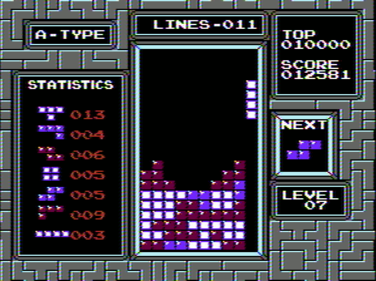
\includegraphics[scale=0.5]{tetris_nes.png}\\

\textbf{Figura 1:} \textit{captura de tela da versão} NES \textit{do jogo}
\end{center}

\subsubsection{Complexidade computacional}
Foi provado \cite{b2} que em uma versão de Tetris onde o jogador já conhece toda a sequência de peças que virão, os seguinte objetivos são problemas NP-Completos:
\begin{itemize}
\item Maximizar o número de linhas limpas enquanto joga com a sequência dada;

\item Maximizar o número de peças colocadas antes de completar uma linha;

\item Maximizar o número de pontuações simultâneas de quatro linhas;

\item Minimizar a altura da última peça colocada em uma sequência.

\end{itemize}

Com exceção do terceiro, todos esses objetivos também são difíceis de serem aproximados. 

\subsection{Algoritmos genéticos}
Um algoritmo genético é uma técnica para encontrar uma solução ideal ou próxima à ideal para um problema computacional, com inspirações nas teorias darwinistas de evolução dos seres vivos. As interações do algoritmo são sobre as gerações, onde uma geração é um conjuto de indivíduos e indivíduos são funções/modelos. Em síntese, um algoritmo genético funciona da seguinte maneira \cite{b3}:

\begin{enumerate}
\item Os parâmetros dos indivíduos da primeira geração são gerados randomicamente;

\item Algum tipo de função de custo é aplicada para avaliar cada indivíduo. Essa função é usada para determinar o sucesso dos indivíduos;

\item Alguma porcentagem dos melhores indivíduos (segundo seus resultados do item anterior) é escolhida.

\item Os indivíduos escolhidos no item anterior serão os "pais" da nova geração. A partir deles, combinações e mutações irão gerar os outros indivíduos da nova geração.

\item Repita os passos 2-4 até alguma condição de parada for atingida. Quando isso acontecer retorna o melhor indivíduo da última geração.

\end{enumerate}


\subsection{Redes neurais artificiais}
Rede neural artificial é uma coleção de unidades chamadas neurônios que são interligados entre si com uma ordem (camadas), com inspiração biológica no funcionamento do cérebro dos animais. Cada neurônio de uma camada se liga a todos os neurônios da anterior (se não for a camada de entrada) e da posterior (se não for a camada de saída). Cada neurônio é ativado de acordo com uma função de ativação, os parâmetros dessa função de ativação são as saídas dos neurônios anteriores multiplicados por um peso nas arestas que conectam estes neurônios. Nos neurônios de entrada são inseridos metadados e nas funções de saída algum tipo de resposta ou classificação \cite{b4}.\\

\subsection{Aprendizado de máquina para jogos eletrônicos}

\subsection{Trabalhos relacionados}

\section{Soluções propostas}

\section{Conclusão}

\section{Estudos futuros}

\begin{thebibliography}{00}

\bibitem{b1} \texttt{ \url{http://www.atarihq.com/tsr/special/tetrishist.html}}

\bibitem{b2} Demaine, E. D., Hohenberger, S., \& Liben-Nowell, D. (2003, July). Tetris is hard, even to approximate. In COCOON (pp. 351-363).

\bibitem{b3} Goldberg, D. E. (1989). Genetic Algorithms in Search, Optimization, and Machine Learning.

\bibitem{b4}  Geron, A. (2017). \textit{Hands-on machine learning with Scikit-Learn and TensorFlow: concepts, tools, and techniques to build intelligent systems.}

\end{thebibliography}

\end{document}
